\chapter{Spatial Expressions In Image Descriptions}
\label{sec:spatial}


The importance of spatial language is embedded in fundamental domain questions about parsing visual sensory inputs into meaningful representations. 
In its purest form, the individuation of objects would be a spatial cognition task; 
to recognise where objects begin and where they end in space, how their parts are spatially composed and how the spatial properties (including shapes and locations) interact with each other.  
In chapter 1, we stated that the use cases of grounded language generation and understanding brought us to the study of spatial language. In a large body of work on referring expression generation 
\citep{DaleReiter:1995,Krahmer:2011aa} with applications that describe scenes \citep{Viethen:2008aa} and images  \citep{Mitchell:2012aa,elliott2013image}, describe visible objects  \citep{mitchell-etal-2013-generating} and engage in human-robot dialogue \citep{kelleher-kruijff-2006-incremental,Dobnik:2009dz}, spatial grounding language is inseparable from the tasks. 
In this chapter, we discuss the relevant topics and concepts regarding how human language can describe the space, the location of objects and the relation between them in an image.

\section{Spatial expressions}
\label{sec:spatial:expressions}
There are many ways to describe a situation and convey information about the location of important matters. The most direct form of denoting the location of objects in natural language is to use \emph{locative expressions}. 
The simplest type of locative expression is composed of three constituents \textemdash  a locative preposition and two noun phrases.
One of the noun phrases is the subject of the preposition and the other is the object. 
\begin{figure}[t]
	\centering
	\begin{minipage}{0.6\linewidth}
		\begin{itemize}[leftmargin=0.1cm,itemsep=1em]
			\item[] The~\textit{frog~next~to}~the~\textit{pond}.
			\item[] The~\textit{frog}~is~\textit{next~to}~the~\textit{pond}.
			\item[] There~is~a~\textit{frog~next~to}~the~\textit{pond}.
			\item[] The~\textit{frog~next~to}~the~\textit{pond}~is~watching~us.
		\end{itemize}
	\end{minipage}%
	\begin{minipage}{0.4\linewidth}
		\centering
		\fbox{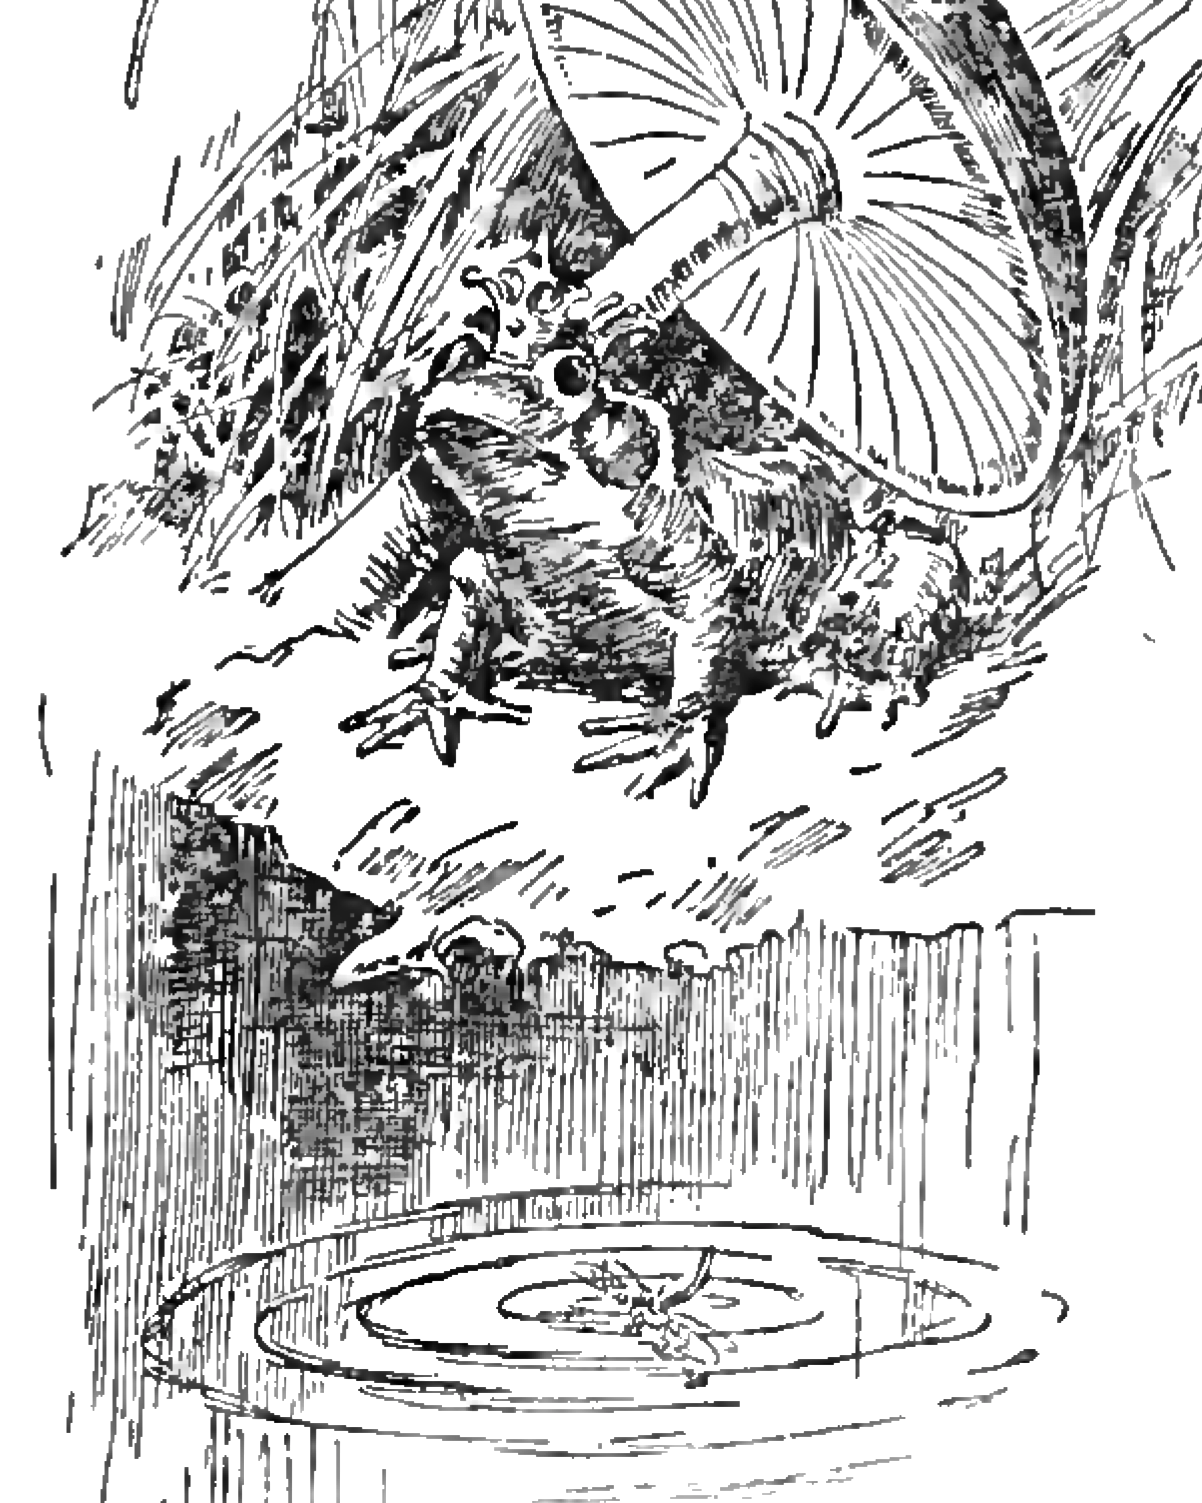
\includegraphics[width=0.78\linewidth]{gfx/frog-prince.png}\footnote{The drawing from \emph{Grimm's Fairy Tales} by \cite{grimmsfairytales1899}}}
	\end{minipage}%
	\caption{Describing the location of target and landmark \textemdash  $\langle$ \textit{frog},\textit{next~to},\textit{pond}$\rangle$.}\label{fig:frog-next-to-pond}
\end{figure}
For example, in `the~frog~next~to~the~pond' the preposition  `next~to' describes the location of the subject `the~frog' with respect to the object `the~pond'. The subject/object are also known by different names, such as \emph{referent}/\emph{relatum} \citep{Miller-JohnsonLaird:1976}, \emph{figure}/\emph{ground} \citep{Talmy:1983} or \emph{located object}/\emph{reference object} \citep{herskovits1986language,Gapp:1994:BasicMeanings,Dobnik:2009dz}.
In this work, we refer to them as  \textsc{Target}/\textsc{Landmark}. 
When referring to a situation with the structure  $\langle\textsc{Target},\textsc{Relation},\textsc{Landmark}\rangle$, 
the expression may be combined with a copulative verb, an existential quantifier or other additional information  (Figure~\ref{fig:frog-next-to-pond}).

In English, there are a small class of words with meanings that denote spatial relations between targets and landmarks. This includes simple words (\emph{on}, \emph{in}, \emph{over}, \emph{under}) and compound phrases (\emph{on top of}, \emph{to the left of}, \emph{to the right of}, \emph{in front of}, and etc.)
Some of these relations are compositional, which means they can be combined to produce new relations (\emph{above} and \emph{far from}). 
Based on the list of prepositions in \citep{landau1993whence}
and alternative compositional and compound relations discussed in  \cite[p.~156]{herskovits1986language}, we created a dictionary of $75$ spatial relations. Considering their alternative forms, with a minor difference in their spatial sense, they constitute $1,194$ entries\footnote{The source code to generate the collection of multi-words expressions is available in the online repository of published studies including \url{https://github.com/GU-CLASP/functional-geometric-lm}.} (Table~\ref{tab:ch2:vocab}). 
For example, `\emph{to the left of}' could be one form of several possible alternative multi-words with close spatial meaning:
\begin{itemize}[topsep=0em,itemsep=0em,partopsep=0em,parsep=0em]
	\item \emph{\{at/on/in/to/by\} the left \{\{hand\} side\} of} $\to$ \emph{to the left of}. 
\end{itemize}

	
\begin{table}[t]
	\begin{tabular}{|lllll|}
		\hline
		about         & above         & across        & after         & afterward     \\
		against       & ago           & along         & alongside     & amid          \\
		among         & apart         & around        & at            & away          \\
		back          & backward      & before        & behind        & below         \\
		beneath       & beside        & between       & bottom        & by            \\
		down          & downstairs    & downward      & during        & east          \\
		from          & front         & here          & in            & inside        \\
		into          & inward        & left          & near          & nearby        \\
		next          & north         & off           & on            & onto          \\
		out           & outside       & outward       & over          & parallel      \\
		perpendicular & right         & side          & sideways      & since         \\
		south         & there         & through       & throughout    & to            \\
		together      & top           & toward        & under         & underneath    \\
		until         & up            & upon          & upstairs      & upward        \\
		via           & west          & with          & within        & without       \\
		\hline
	\end{tabular}
	\vspace{0.5em}
	\caption{The vocabulary of $75$ spatial relations from \cite{landau1993whence} and \cite{herskovits1986language}.}\label{tab:ch2:vocab}
\end{table}


\section{Functional/geometric meaning}
\label{sec:spatial:functional}
Expressing location and describing space is not limited to the prepositional relations in spatial expressions. Other verbs in referring expressions can indicate the relative location between subject and object. With different degrees, these relations might have a strong or weak association with the location of the subject and object. 
For example, `\emph{ride}' entails a specific spatial configuration between the subject and the object, depending on their shape. 
Other relations, such as `\emph{touch}', `\emph{sit on}', and `\emph{jump over}' indicate a specific spatial configuration of subject and object.
Nevertheless, their direct meaning is not just the location of objects; it indicates other kinds of relations, which consequently entail specific spatial arrangements. 

In the same way, the meaning of spatial prepositions is not purely geometrical; it entails other relations and associations between subject and object that are functional. 
The relation  `\emph{over}' does not just describe a geometric location; it also indicates a function \textemdash  the subject provides protection or shelter for the object/s.
The functional sense of relations includes specific interactive relations between entities that are not dependent on the location and spatial configurations.

A simple representation of the geometric sense of relations is based on the acceptability ratings of individual locations with respect to the landmark. 
\cite{logan1996computational} suggest that the mental representation of a geometric meaning could be a template projection of locations on a map, where the landmark is in the middle and each location has its degree of acceptability for the target object. 
A study on location acceptabilities for different prepositions shows that each spatial preposition has a different degree of dependency on object-specific relations  \citep{coventry2001interplay}.
The meaning of each relation is an interplay between the functional and geometric relations of two objects.
For instance, \emph{`above'} has both geometric locational meaning and functional sense. 
When it is used in different context it can have different degree of functional and geometric acceptability.
Spatial relations in natural language have a spectrum of geometricity, with different degree of favouring geometric bias or functional bias. 
Another way to study the object-specific sense of relations is to consider the distributional dependency between relations and objects in image descriptions \citep{Dobnik:2013aa,Dobnik:2014ab}.
In our studies, we consider these aspects of by examining language models.

\section{Image descriptions}
\label{sec:spatial:image}
In a simple \emph{show-and-tell} task, when provided an image, the agent must generate a description of the image. 
Since the early works on human-robot interactions, this task became the centre of interests for natural language grounding \citep{roy2002learning}. 
In recent years, several large datasets have been developed, in which crowd-sourced human annotators describe images from freely available datasets of photographed scenes over the Internet.

\paragraph{Datasets}
Common datasets of image caption tasks, such as MSCOCO  \citep{lin2014microsoft} with more than 300,000 images and Flickr30k  \citep{flickr30k} with 30,000 images, each provide five alternative descriptions per image. 
However, the variation and number of geometric spatial relations in the dataset is limited;
`\emph{to the left of}' and `\emph{to the right of}' are rarely used in the dataset. 
On the other hand, the Visual Genome \citep{krishna2017visual} provides 50 region descriptions and triplet annotations per image, for a total of over 108,000 images. 
The annotation schema, in this case, was slightly different from captioning, as it asks annotators to describe specific parts of the images or the relation between two object areas in the images. 
In this dataset, description and relation annotations are associated with relevant bounding boxes in the image.


\paragraph{Grounding spatial descriptions}
Both generating and understanding a spatial description with three components \textemdash  $\textsc{Target}$, $\textsc{Relation}$, $\textsc{Landmark}$ \textemdash  requires several types of knowledge:
 (1) object identification,
 (2) comprehension of geometric configuration,
 (3) capturing object-specific relations between objects and 
 (4) a frame of reference for projective relations `\emph{to the right of}' and `\emph{below}'.
When people describe image contents, they commonly use spatial expressions. 
A scene can be described correctly using any spatial relation fitting the same objects depending on the intent of the speaker.
However, the image description task may use the knowledge about the scene in a specific way.%
Precisely, object identification and the capture of object-specific relations in the picture might be enough to describe an image with spatial expressions.

\section{Summary}
\label{sec:spatial:summary}
In this chapter, we described the concept of locative expressions and its connection with image descriptions. 
Spatial relations denote locations in scenes. However, their meaning, to some extent, is also dependent on object-specific relations. 
In our studies on grounding spatial descriptions, we will use datasets of images with descriptions, including MSCOCO\citep{lin2014microsoft}, Flickr30k\citep{flickr30k} and Visual Genome \citep{krishna2017visual}.